\chapter{Introduction to Vericert}%
\label{sec:introduction-to-vericert}

\begin{chapsummary}
  This chapter describes the main architecture of the HLS tool, and the way in
  which the Verilog back end was added to \compcert{}.  This chapter also covers
  an example of converting a simple C program into hardware, expressed in the
  Verilog language.  \Cref{sec:itv:unreliability-hls} is based on a short paper
  coauthored with Zewei Du, Nadesh Ramanathan, and John
  Wickerson~\cite{herklotz21_esrhlst}.  The rest of the chapter, together with
  \cref{sec:trusted-computing-base}, is based on a paper coauthored with James
  D. Pollard, Nadesh Ramanathan, and John Wickerson~\cite{herklotz21_fvhls}.
\end{chapsummary}

\section{Unreliability of High-Level Synthesis}%
\label{sec:itv:unreliability-hls}

Are \gls{HLS} tools reliable? Questions have been raised about the reliability
of HLS before; for example, Andrew Canis, co-creator of the LegUp HLS tool,
wrote that \textquote[{\textcite[Section 3.4.6]{canis15_legup}}]{high-level
  synthesis research and development is inherently prone to introducing bugs or
  regressions in the final circuit functionality}.  In this section, I
investigate whether there is substance to this concern by conducting an
empirical evaluation of the reliability of several widely used HLS tools.

The approach used is called \emph{fuzzing}.  This is an automated testing method
in which randomly generated programs are given to compilers to test their
robustness~\cite{chen13_tcf, sun16_tucbgl, liang18_f, zhang19_fubsmc,
  yang11_findin_under_bugs_c_compil, lidbury15_many_core_compil_fuzzin}.  The
generated programs are typically large and rather complex, and they often
combine language features in ways that are legal but counter-intuitive; hence
they can be effective at exercising corner cases missed by human-designed test
suites.  Fuzzing has been used extensively to test conventional compilers; for
example, \textcite{yang11_findin_under_bugs_c_compil} used it to reveal more
than three hundred bugs in GCC and LLVM, and tested CompCert as well, only
finding bugs in the verified parts of the code.

\begin{example}[A miscompilation bug in Vivado HLS]
\label{ex:vivado_miscomp}
Figure~\ref{fig:vivado_bug1} shows a program that produces the wrong result
during hardware simulation in Xilinx Vivado HLS v2018.3, v2019.1 and
v2019.2.\footnote{This program, like all the others in this paper, includes a
  \texttt{main} function, which means that it compiles straightforwardly with
  GCC. To compile it with an HLS tool, I rename \texttt{main} to
  \texttt{result}, synthesise that function, and then add a new \texttt{main}
  function as a testbench that calls \texttt{result}.} The program repeatedly
shifts a large integer value \texttt{x} right by the values stored in array
\texttt{arr}.  Vivado HLS returns \texttt{0x006535FF}, but the result returned
by GCC (and subsequently confirmed manually to be the correct one) is
\texttt{0x046535FF}. The bug was initially revealed by a randomly generated
program of around 113 lines, which was reduced to the minimal example shown in
the figure.  I reported this issue to Xilinx, who confirmed it to be a
bug.\footnote{\url{https://web.archive.org/web/20210419185153/https://forums.xilinx.com/t5/High-Level-Synthesis-HLS/Issue-with-shift-in-for-loop/m-p/1170197}}
\end{example}

\begin{figure}
\centering
\begin{minipage}{6cm}
\begin{minted}{c}
unsigned int x = 0x1194D7FF;
int arr[6] = {1, 1, 1, 1, 1, 1};

int main() {
  for (int i = 0; i < 2; i++)
    x = x >> arr[i];
  return x;
}
\end{minted}
\end{minipage}
\caption[Miscompilation bug in Xilinx Vivado HLS v2018.3, v2019.1 and
v2019.2.]{Miscompilation bug in Xilinx Vivado HLS. The generated hardware
  returns \texttt{0x006535FF} but the correct result is \texttt{0x046535FF}.}%
\label{fig:vivado_bug1}
\end{figure}

\def\totaltestcases{6700}
\def\totaltestcasefailures{1191}
\def\numuniquebugs{8}
\def\vivadotestcases{3645}

The fuzzer used Csmith to randomly generate C code and modified it to make it
suitable for HLS tools.  For example, pointers had to be removed because some
cases, like pointers of other pointers, are explicitly not supported by Vivado
HLS.  I tested the following \gls{HLS} tools: Intel i++ 18.1, LegUp 4.0, Bambu
0.9.7 and Xilinx Vivado HLS v2018.3, v2019.1 and v2019.2.
\Cref{fig:existing_tools} shows an Euler diagram of our results.  We see that
918 (13.7\%), 167 (2.5\%), 83 (1.2\%) and 26 (0.4\%) test-cases fail in Bambu,
LegUp, Vivado HLS and Intel i++ respectively.  The bugs I reported to the Bambu
developers were fixed during our testing campaign, so I also tested the
development branch of Bambu (0.9.7-dev) with the bug fixes, and found only 17
(0.25\%) failing test-cases remained.  Although i++ has a low failure rate, it
has the highest time-out rate (540 test-cases) due to its remarkably long
compilation time. No other tool had more than 20 time-outs.  Note that the
absolute numbers here do not necessarily correspond to the number of bugs in the
tools, because a single bug in a language feature that appears frequently in our
test suite could cause many failures.  Moreover, I am reluctant to draw
conclusions about the relative reliability of each tool by comparing the number
of failures, because these numbers are so sensitive to the parameters of the
randomly generated test suite used. In other words, I can confirm the
\emph{presence} of bugs, but cannot deduce the \emph{number} of them (nor their
importance).

In total, I found at least \numuniquebugs{} unique bugs across all the tools,
including both crashes and miscompilations.  Conventional compilers have become
quite resilient to fuzzing over the last decade, so recent work on fuzzing
compilers has had to employ increasingly imaginative techniques to keep finding
new bugs~\cite{even-mendoza20_ce}.  In contrast, I have found that HLS tools can
be made to exhibit bugs even using the relatively basic fuzzing techniques.
This motivates the need for a verified \gls{HLS} tool.

\definecolor{intel}{HTML}{66c2a5}
\definecolor{vivado}{HTML}{fc8d62}
\definecolor{legup}{HTML}{8da0cb}
\definecolor{bambu}{HTML}{e78ac3}
\definecolor{bambudev}{HTML}{bf8be8}
\definecolor{timeout}{HTML}{ef4c4c}
\begin{figure}
  \centering
    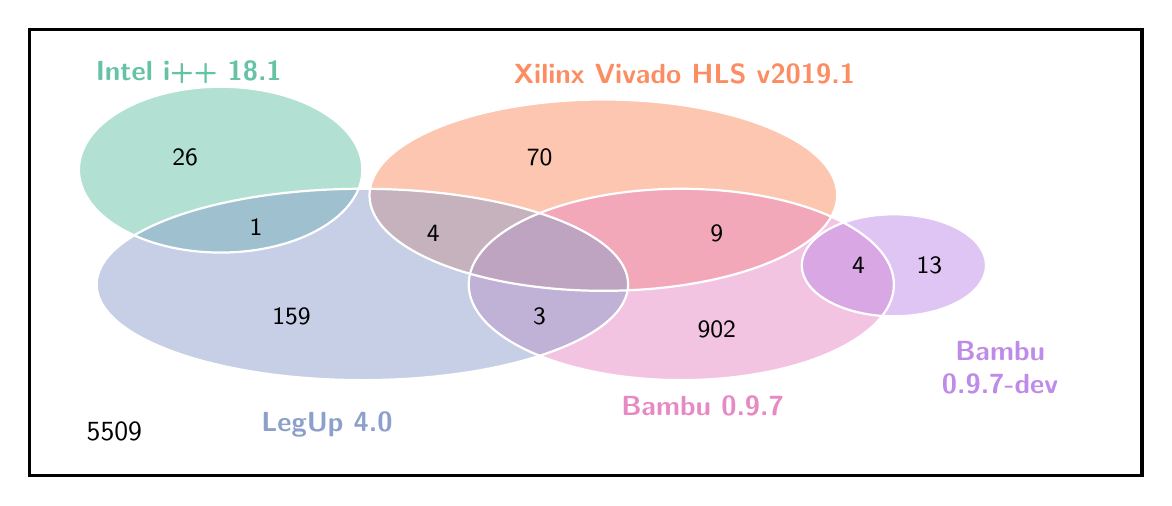
\begin{tikzpicture}[scale=0.9,yscale=0.9,font=\sffamily]
      \draw[very thick] (-7.2,7.0) rectangle (8.5,0);
      \fill[vivado,fill opacity=0.5] (0.9,4.4) ellipse (3.3 and 1.5);
      \fill[intel,fill opacity=0.5] (-4.5,4.8) ellipse (2.0 and 1.3);
      \fill[bambu,fill opacity=0.5] (2,3) ellipse (3 and 1.5);
      \fill[bambudev,fill opacity=0.5] (5,3.3) ellipse (1.3 and 0.8);
      \fill[legup,fill opacity=0.5] (-2.5,3) ellipse (3.75 and 1.5);
      \draw[white, thick] (0.9,4.4) ellipse (3.3 and 1.5);
      \draw[white, thick] (-4.5,4.8) ellipse (2.0 and 1.3);
      \draw[white, thick] (2,3) ellipse (3 and 1.5);
      \draw[white, thick] (5,3.3) ellipse (1.3 and 0.8);
      \draw[white, thick] (-2.5,3) ellipse (3.75 and 1.5);
      \node[align=center, anchor=south west] at (-0.5,6) {\textcolor{vivado}{\textbf{Xilinx Vivado HLS v2019.1}}};
      \node[anchor=south west] at (-6.4,6) {\textcolor{intel}{\textbf{Intel i++ 18.1}}};
      \node at (-3,0.8) {\textcolor{legup}{\textbf{LegUp 4.0}}};
      \node at (2.3,1.1) {\textcolor{bambu}{\textbf{Bambu 0.9.7}}};
      \node[align=center] at (6.5,1.7) {\textcolor{bambudev}{\textbf{Bambu}} \\ \textcolor{bambudev}{\textbf{0.9.7-dev}}};
      \node at (-3.5,2.5) {\small 159};
      \node at (-5,5) {\small 26};
      \node at (-4,3.9) {\small 1};
      \node at (-1.5,3.8) {\small 4};
      \node at (0,2.5) {\small 3};
      \node at (2.5,2.3) {\small 902};
      \node at (2.5,3.8) {\small 9};
      \node at (0,5) {\small 70};
      \node at (4.5,3.3) {\small 4};
      \node at (5.5,3.3) {\small 13};
      \node at (-6,0.7) {5509};
    \end{tikzpicture}
    \caption[The number of failures per tool.]{The number of failures per tool
      out of \totaltestcases{} test-cases. Overlapping regions mean that the
      same test-cases failed in multiple tools.}\label{fig:existing_tools}
\end{figure}

\section{Main Design Decisions of Vericert}%
\label{sec:itv:main-design-decisions}

Our solution to the reliability problem in \gls{HLS} is Vericert, a formally
verified \gls{HLS} tool.  First, I will describe the main design decisions
behind Vericert in \cref{sec:itv:main-design-decisions} and I will then give an
example of a translation from C code into Verilog through Vericert in
\cref{sec:itv:translating-c-to-verilog}.

\paragraph{Choice of source language}

C was chosen as the source language as it remains the most common source
language amongst production-quality HLS tools~\cite{canis13_l,
  amd23_vitis_high_synth, intel20_hsc, pilato13_bambu}. This, in turn, may be
because it is \textquote[{\textcite{gajski10_what_hls}}]{[t]he starting point
  for the vast majority of algorithms to be implemented in hardware}, lending a
degree of practicality.  The availability of
\compcert{}~\cite{leroy09_formal_verif_realis_compil} also provides a solid
basis for formally verified C compilation.  Since a lot of existing code for HLS
is written in C, supporting C as an input language, rather than a custom
domain-specific language, means that \vericert{} is more practical.  I
considered Bluespec~\cite{nikhil04_bsv}, but decided that although it
\textquote[{\textcite{greaves19_resear_note}}]{can be classed as a high-level
  language}, it is too hardware-oriented to be suitable for traditional HLS.  I
also considered using a language with built-in parallel constructs that map well
to parallel hardware, such as occam~\cite{page91_compil_occam},
Spatial~\cite{koeplinger18_s} or Scala~\cite{bachrach12_chisel}.

\paragraph{Choice of target language}

Verilog was chosen as the output language for \vericert{} because it is one of
the most popular HDLs and there already exist a few formal semantics for it that
could be used as a target~\cite{lööw19_verif_compil_verif_proces,
  meredith10_veril}.  Bluespec, previously ruled out as a source language, is
another possible target and there exists a formally verified translation to
circuits of variants of Bluespec using K\^{o}ika~\cite{bourgeat20_essen_blues}
or Fe-Si~\cite{braibant13_formal_verif_hardw_synth}.  However, Bluespec is
mainly targeted at being a source language for hardware design and would present
similar challenges to targeting a language like Verilog from a software
language.

% \JP{This needs an extra comment maybe?}\YH{Maybe about bluespec not being an
% ideal target language because it's quite
% high-level?} % but targeting this language would not be trivial as it is not meant to be targeted by an automatic tool, instead strives to a formally verified high-level hardware description language instead.

%\JW{Can we mention one or two alternatives that we considered? Bluespec or Chisel or one of Adam Chlipala's languages, perhaps?}

\paragraph{Choice of implementation language}

I chose Coq as the implementation language because of its mature support for
code extraction; that is, its ability to generate OCaml programs directly from
the definitions used in the theorems.
\compcert{}~\cite{leroy09_formal_verif_realis_compil} was chosen as the front
end because it has a well established framework for simulation proofs about
intermediate languages, and it already provides a validated C
parser~\cite{jourdan12_valid_lr_parser}.  The Vellvm
framework~\cite{zhao12_formal_llvm_inter_repres_verif_progr_trans} was also
considered because several existing HLS tools are already LLVM-based, but
additional work would be required to support a high-level language like C as
input.  The .NET framework has been used as a basis for other HLS tools, such as
Kiwi~\cite{greaves08_kiwi}, and LLHD~\cite{schuiki20_llhd} has been recently
proposed as an intermediate language for hardware design, but neither are
suitable for us because they lack formal semantics.

\begin{figure}
  \centering
  \begin{tikzpicture}
    [font=\strut\sffamily]
    \node[ir] (compcertc) {CompCert C};
    \node[right=2cm of compcertc] (frontend) {};
    \begin{pgfonlayer}{background}
          \node[bgbox,fill=bgbox1,minimum height=4cm,minimum width=3cm,yshift=3mm]
    (frontendbg) at (frontend) {};
    \end{pgfonlayer}
    \node[pass] (frontendpass) at (frontend) {$\vphantom{A}\cdots$};
    \node[right=3.5cm of frontend] (rtlghost) {};
    \begin{pgfonlayer}{background}
      \node[bgbox,fill=bgbox2,minimum height=4cm,minimum width=3cm,yshift=3mm]
      (rtlghostbg) at (rtlghost) {};
    \end{pgfonlayer}
    \node[ir,below=2mm of rtlghost,xshift=-8mm] (rtl) {\rtl{}};
    \node[pass,right=5mm of rtl] (rtlpass) {$\vphantom{A}\cdots$};
    \node[pass,above=2mm of rtlghost] (opts) {optimisations};
    \node[anchor=south,above=2mm of opts] (backend) {Back End};
    \node[ir,right=2cm of rtlghost] (nativecode) {Native Code};
    \path (backend) -| node {Front End} (frontend);
    \draw[ed] (compcertc) -- (frontendpass) -- ++(2cm,0) |- (rtl);
    \draw[ed] (rtl) -- (rtlpass) -- ++(1cm,0) |- (nativecode);
    \draw[very thick] (opts) to [out=310,in=20] (rtl);
    \draw[edr] (rtl) to [out=90,in=220] (opts);
    \node[pass,below=2.3cm of compcertc,xshift=1cm] (findbb) {find\\basic blocks};
    \node[ir,right=of findbb] (rtlblock) {\rtlblock{}};
    \draw[ed] (rtlblock) to [out=300,in=240,loop,looseness=10] (rtlblock);
    \node[pass,right=of rtlblock] (schedule) {schedule};
    \node[pass,below=of rtlblock] (ifconv) {if-conversion};
    \node[ir,right=of schedule] (rtlpar) {\rtlpar{}};
    \node[pass,below=of findbb,yshift=-2cm,xshift=-1cm] (hyperblock destruction) {hyperblock\\destruction};
    \node[ir,right=of hyperblock destruction] (rtlsubpar) {\rtlsubpar{}};
    \node[pass,right=of rtlsubpar] (htl generation) {\htl{} \\
      generation};
    \node[ir,right=of htl generation] (htl) {\htl{}};
    \node[pass,right=of htl] (bram insertion) {BRAM \\ insertion};
    \node[ir,below=of bram insertion] (htlmem) {\htl{}};
    \node[pass,left=of htlmem] (forward substitution) {forward \\ substitution};
    \node[ir,left=of forward substitution] (htlsubst) {\htl{}};
    \node[pass,left=of htlsubst] (verilog generation) {verilog \\ generation};
    \node[ir,left=of verilog generation] (verilog) {Verilog};

    \begin{pgfonlayer}{background}
      \node[bgbox,fit={(findbb)(rtlblock)(ifconv)(rtlpar)}] (schedulebox) {};
      \node[bgbox,fit={(hyperblock destruction)(bram
        insertion)(htlmem)(forward substitution)(verilog)}] (hardwaregenbox) {};
    \end{pgfonlayer}

      \path (hardwaregenbox.north west) --
      node[font=\sffamily\small,align=center,rotate=90,yshift=5mm] (hardwaregen label)
      {Hardware Generation\\\Cref{sec:hardware-generation}}
      (hardwaregenbox.south west);
      \path (schedulebox.north west) --
      node[font=\sffamily\small,align=center,rotate=90,yshift=14.5mm] (schedule label)
      {Hyperblock Scheduling\\\Cref{sec:hyperblock-scheduling}}
      (schedulebox.south west);

      \begin{pgfonlayer}{background}
        \node[bgbox,fill=bgbox4,fit={(hyperblock destruction)(bram
          insertion)(htlmem)(forward substitution)(verilog)(hardwaregen label)}]
        (hardwaregenboxb) {};
      \node[bgbox,fill=bgbox3,fit={(findbb)(rtlblock)(ifconv)(rtlpar)(schedule
        label)}] (scheduleboxb) {};
      \filldraw[bgbox,fill=bgbox3] (scheduleboxb.north west) rectangle
      (hardwaregenboxb.north east
      |- scheduleboxb.south east);
      \end{pgfonlayer}

    \path (rtlghostbg.west) -| node[font=\sffamily\small,anchor=south,rotate=90] {CompCert} (hardwaregen label);

    \draw[ed] (rtl) -- ++(0,-1.3cm) -| (findbb) -- (rtlblock);
    \draw[ed] (rtlblock) -- (schedule) -- (rtlpar);
    \draw[ed] (rtlpar) -- ++(0,-2.7cm) -| (hyperblock destruction) -- (rtlsubpar);
    \draw[ed] (rtlsubpar) -- (htl generation) -- (htl);
    \draw[ed] (htl) -- (bram insertion) -- (htlmem);
    \draw[ed] (htlmem) -- (forward substitution) -- (htlsubst);
    \draw[ed] (htlsubst) -- (verilog generation) -- (verilog);

    \node[blacknum] at (findbb.north west) {1};
    \node[blacknum] at (ifconv.north west) {2};
    \node[blacknum] at (schedule.north west) {3};
    \node[blacknum] at (hyperblock destruction.north west) {4};
    \node[blacknum] at (htl generation.north west) {5};
    \node[blacknum] at (bram insertion.north west) {6};
    \node[blacknum] at (forward substitution.north west) {7};
    \node[blacknum] at (verilog generation.north west) {8};
  \end{tikzpicture}
  \caption{\vericert{} as a Verilog back end to \compcert{}.}%
  \label{fig:rtlbranch}
\end{figure}

\paragraph{Architecture of \vericert{}}

An overview of \vericert{}'s workflow is given in \cref{fig:rtlbranch}, which
shows that \vericert{} branches off from \compcert{} at the \rtl{} stage,
followed by a number of transformations related to the scheduling instructions,
and finally transformations that generate the final hardware.

CompCert's \gls{RTL} was selected as the starting point. Branching off
\emph{before} this point (at \gls{CminorSel} or earlier) denies \compcert{} the
opportunity to perform optimisations such as constant propagation and dead-code
elimination, which, despite being designed for software compilers, have been
found useful in HLS tools as well~\cite{cong11_high_level_synth_fpgas}. And if
we branch off \emph{after} this point (at \gls{LTL} or later) then \compcert{}
has already performed register allocation to reduce the number of registers and
spill some variables to the stack; this transformation is not required in HLS
because there are many more registers available, and these should be used
instead of \gls{BRAM} whenever possible.

\rtl{} is also attractive because it is the closest intermediate language to
LLVM \gls{IR}, which is used by several existing HLS compilers.  It has an
unlimited number of pseudo-registers, and is represented as a \gls{CFG} where
each instruction is a node with links to the instructions that can follow it.
\rtl{} does not have the SSA property, however, this is not required for the
translation to hardware and mainly assists the static analysis passes.  One
difference between LLVM \gls{IR} and \rtl{} is that \rtl{} includes operations
that are specific to the chosen target architecture; I chose to target the
x86\_32 back end because it generally produces relatively dense \rtl{} thanks to
the availability of complex addressing modes.  The translation from \rtl{} is
then performed as follows:

\begin{enumerate}[label=\protect\blacknum{\arabic*}]
\item Basic block generation creates basic blocks from the pure \rtl{}
  \gls{CFG}.
\item \Gls{if-conversion} combines basic blocks into a single hyperblock based on
  heuristics on the \gls{CFG} layout.  The hyperblock is represented as a basic
  block of predicated instructions with an exit instruction to leave the basic
  block prematurely.
\item The scheduler itself is written in unverified OCaml and works similarly
  to those in existing HLS tools~\cite[]{canis13_l}: it takes a set of
  scheduling constraints that capture the clock period, available hardware
  resources, and dependencies between operations, encodes them as a
  \glsfirst{SDC}~\cite[]{cong06_sdc}, and then hands them off to a linear
  program solver.  The result is checked by a verified validator that ensures the correctness of the schedule that was produced by the scheduler.
\item Next, the hyperblocks are destroyed to explicitly place instructions into
  individual states.
\item \htl{} is generated, which is a language that models an \gls{FSMD}, which
  is used as an intermediate language that is simpler to manipulate than Verilog
  but is still close enough to a hardware description so that hardware-specific
  optimisations can be performed on it.
\item \gls{BRAM} insertion generates a proper memory interface for any
  interaction with the stack frame.
\item To ensure that these assignments are actually performed in parallel, a
  final pass performs \emph{forward substitution}~\cite[p.~109]{hopwood78_decom}
  to turn the sequence of Verilog blocking assignments into a sequence of
  nonblocking assignments. For example:
%
\begin{center}
\begin{tikzpicture}[>=Latex,shorten >=1pt,label/.style={circle,draw,fill=white,inner sep=0.4mm,font=\footnotesize}, bb/.style={align=left, draw=white, fill=black!5},font=\strut\sffamily]
\node[bb,inner sep=3mm] (initial) {\begin{minipage}{3.5cm}
\begin{minted}{systemverilog}
always @(posedge clk)
  begin
    r = r1 * r2;
    r = r + r3;
    r5 = r + r4;
  end
\end{minted}
\end{minipage}};
\node[right=3.5cm of initial,bb,inner sep=3mm] (scheduled) {%
  \begin{minipage}{5.4cm}
\begin{minted}{systemverilog}
always @(posedge clk)
  begin
    r <= r1 * r2;
    r <= (r1 * r2) + r3;
    r5 <= ((r1 * r2) + r3) + r4;
  end
\end{minted}
  \end{minipage}%
};
\draw[ed] (initial) -- node [pass] {forward\\substitution}
(scheduled);
\end{tikzpicture}
\end{center}
%
The two versions are semantically equivalent, but we find that the second, in
which both right-hand sides must be evaluated before either assignment is
performed, makes the downstream logic synthesis tools more likely to produce the
hardware we intend (which, in this particular example, involves exploiting a
fused multiply--accumulator unit if available).%
\footnote{As the example shows, forward substitution does not remove duplicate
  writes to a variable because Verilog semantics explicitly state that the order
  of nonblocking assignments to the same variable will be
  preserved~\cite[p.~254]{ieee24_iss}.}
\item Finally, syntactic Verilog is generated from \htl{}, which consists of
  translating the \gls{FSMD} into a case statement and implementing the memory
  interface in Verilog.
\end{enumerate}

\section{Translating C to Verilog by Example}%
\label{sec:itv:translating-c-to-verilog}

\Cref{fig:accumulator_c_rtl} illustrates the translation of a simple program
that stores and retrieves a value from an array.  This section describes the
stages of the \vericert{} translation, referring to this program as an example.

\subsection{Translating C to \rtl{}}

The first stage of the translation uses unmodified \compcert{} to transform the
C input, shown in \cref{fig:accumulator_c}, into an \rtl{} intermediate
representation, shown in \cref{fig:accumulator_rtl}.  As part of this
translation, function inlining is performed on all functions, which allows us to
support function calls without having to support the \texttt{Icall} \rtl{}
instruction.  Although the duplication of the function bodies caused by inlining
can increase the area of the hardware, it can have a positive effect on latency
and is therefore a common HLS optimisation~\cite{noronha17_rapid_fpga}.
Scheduling in particular benefits from inlining of function calls so that the
instructions can be scheduled together and larger hyperblocks can be formed.
Inlining precludes support for recursive function calls, but this feature is not
supported in most HLS tools anyway~\cite{thomas16_srcht}.

\begin{figure}
  \centering
    \begin{subfigure}[b]{0.48\linewidth}
\begin{minted}[fontsize=\footnotesize,linenos,xleftmargin=20pt]{c}
int main(int i) {
    int x[2] = {3, 6};
    return x[i];
}
\end{minted}
      \caption{Example C code passed to \vericert{}.}\label{fig:accumulator_c}
    \end{subfigure}\hfill%
    \begin{subfigure}[b]{0.48\linewidth}
%\begin{minted}[fontsize=\footnotesize,linenos,xleftmargin=20pt]{c}
\lstset{numbers=left,basicstyle=\footnotesize\ttfamily,numberstyle=\tiny,keepspaces=true,showspaces=true,xleftmargin=20pt}
\begin{rtllisting}
main(r1) {
  7: r5 := 3
  6: M[&Stack[0]] := r5
  5: r4 := 6
  4: M[&Stack[4]] := r4
  3: r3 := &Stack[0]
  2: r2 := M[r3 + r1 * 4 + 0]
  1: return r2
}
\end{rtllisting}
%\end{minted}
      \caption{\rtl{} produced by the \compcert{} front end without any optimisations.}\label{fig:accumulator_rtl}
    \end{subfigure}
    \caption{Translating a simple program from C to \rtl{}.}\label{fig:accumulator_c_rtl}
\end{figure}

\subsection{Scheduling \rtl{} instructions}

The first step in the translation performed by Vericert is to schedule the
instructions according to the resource constraints imposed by the hardware
target.  An example of such a constraint is that two memory operations cannot be
performed in the same cycle.  The goal is to schedule as many instructions as
possible together to give the scheduler the most flexibility.  Vericert
therefore constructs hyperblocks from the \rtl{} \gls{CFG}, by building basic
blocks first and then performing \gls{if-conversion} on blocks that should be merged.
This is shown in \cref{fig:accumulator_seq}, where all the instructions can fit
into a single basic block.  Each hyperblock can then be scheduled individually
using \gls{SDC} scheduling by specifying any necessary constraints, the result
of which is shown in \cref{fig:accumulator_par}, where one can see that
instructions with dependencies have been separated into different states and
instructions that can execute in parallel are placed into the same state.  Each
memory operation is placed into its own state.  The instructions are placed into
additional bundles, designated by parentheses, which could contain additional
operations that are chained sequentially within one clock cycle.

The \gls{SDC} scheduling algorithm itself is unverified but a verified validator
checks the resulting schedule against the unscheduled program.  This makes it
possible to change heuristics in the scheduler without it affecting the proof.
The scheduled program language is called \rtlpar{} and specifies in which cycle
each instruction will be executed.  \rtlpar{} however still contains the
coarse-grained structure of hyperblocks, so this structure is destroyed to
produce \rtlsubpar{}, shown in \cref{fig:accumulator_par}.  The representation
is still hardware agnostic even if the current implementation of the scheduler
is specific to an \gls{FPGA} target, and therefore supports all \rtl{}
instructions.  Details about the scheduler and proof of correctness are given in
\cref{sec:hyperblock-scheduling}.  This representation is then ready to be
translated into hardware.

\begin{figure}
  \centering
    \begin{subfigure}[b]{0.48\linewidth}
%\lstset{numbers=left{basicstyle=\small\ttfamily,keepspaces=true,showspaces=true}}
%\begin{rtllisting}
%\begin{minted}[fontsize=\footnotesize,linenos,xleftmargin=20pt]{c}
\lstset{numbers=left,basicstyle=\footnotesize\ttfamily,numberstyle=\tiny,keepspaces=true,showspaces=true,xleftmargin=20pt}
\begin{rtllisting}
main(r1) {
  7: {
    r5 := 3
    M[&Stack[0]] := r5
    r4 := 6
    M[&Stack[4]] := r4
    r3 := &Stack[0]
    r2 := M[r3 + r1 * 4 + 0]
    return r2
  }
}
\end{rtllisting}
%\end{minted}
      \caption{Code in \rtlblock{} after basic blocks have been generated.}\label{fig:accumulator_seq}
    \end{subfigure}\hfill%
    \begin{subfigure}[b]{0.48\linewidth}
%\begin{minted}[fontsize=\footnotesize,linenos,xleftmargin=20pt]{c}
\lstset{numbers=left,basicstyle=\footnotesize\ttfamily,numberstyle=\tiny,keepspaces=true,showspaces=true,xleftmargin=20pt}
\begin{rtllisting}
main(r1) {
  7: {
    r5 := 3
    r4 := 6
    r3 := &Stack[0]
    goto 13
  }
  13: {
    M[&Stack[0]] := r5
    goto 14
  }
  14: {
    M[&Stack[4]] := r4
    goto 15
  }
  15: {
    r2 := M[r3 + r1 * 4 + 0]
    goto 16
  }
  16: { return r2 }
}
\end{rtllisting}
%\end{minted}
      \caption{\rtlsubpar{} code produced after scheduling and hyperblock destruction.}\label{fig:accumulator_par}
    \end{subfigure}
    \caption{Scheduling a simple program from \rtlblock{} to
      \rtlpar{}.}\label{fig:accumulator_gblseqpar}
\end{figure}

% + TODO Explain the main mapping in a short simple way

% + TODO Clarify connection between CFG and FSMD

% + TODO Explain how memory is mapped \JW{I feel like this could use some sort
% of citation, but I'm not sure what. I guess this is all from "Hardware Design
% 101", right?}\YH{I think I found a good one actually, which goes over the
% basics.}  \JW{I think it would be worth having a sentence to explain how the C
% model of memory is translated to a hardware-centric model of memory. For
% instance, in C we have global variables/arrays, stack-allocated
% variables/arrays, and heap-allocated variables/arrays (anything else?). In
% Verilog we have registers and \gls{BRAM} blocks. So what's the correspondence
% between the two worlds?  Globals and heap-allocated are not handled,
% stack-allocated variables become registers, and stack-allocated arrays become
% \gls{BRAM} blocks? Am I close?}\YH{Stack allocated variables become \gls{BRAM}
% as well, so that we can deal with addresses easily and take addresses of any
% variable.} \JW{I see, thanks. So, in short, the only registers in your
% hardware designs are those that store things like the current state, etc. You
% generate a fixed number of registers every time you synthesis -- you don't
% generate extra registers to store any of the program variables. Right?}

% \JP{I've become less comfortable with this term, but it's personal preference
% so feel free to ignore. I think `generalised finite state machine' (i.e.\
% thinking of the entire `data-path' as contributing to the overall state) is
% more accurate.}\YH{Hmm, yes, I mainly chose FSMD because there is quite a lot
% of literature around it.  I think for now I'll keep it but for the final draft
% we could maybe change it.}  This means that the state transitions can be
% translated into a simple finite state machine (FSM) where each state contains
% data operations that update the memory and registers.

\subsection{Translating \rtlpar{} to \htl{}}\label{sec:itv:rtlpar-to-htl}

The next translation is from \rtlpar{}, the program formed of scheduled
hyperblocks, to an intermediate hardware translation language (\htl{}).  This
translation involves going from a \gls{CFG} representation of the computation to
an \gls{FSMD} representation~\cite{hwang99_ffplp}. An \gls{FSMD} is a
generalised state machine where the state is supplemented by registers and
memory that can store results of computations.  \Cref{fig:accumulator_diagram}
shows the resulting \gls{FSMD} architecture for the running example. The
right-hand block is the control logic that computes the next state, while the
left-hand block updates all the registers and \gls{BRAM} based on the current
program state.  However, in general the state machine cannot be separated from
the data path completely, because state updates may depend on computations in
the data path and on the value of registers.  Hence, an \htl{} program consists
of a map from states to Verilog statements, which describe updates done to both
the state register as well as other registers and interact with memory.

The \htl{} language was mainly introduced to simplify the proof of translation
from \rtl{} to Verilog, as these languages have very different semantics.  It
serves as an intermediate language with similar semantics to \rtl{} at the top
level, using maps to represent what to execute at every state, and similar
semantics to Verilog at the lower level because it already uses Verilog
statements instead of more abstract instructions to perform computations.  The
next state is also computed explicitly in each state by modifying the state
register.  Compared to plain Verilog and due to using maps to represent the
Verilog statement that should execute at every state, \htl{} is simpler to
manipulate and analyse, thereby making it easier to prove optimisations like
\gls{BRAM} insertion.

\begin{figure}
  \centering
\definecolor{control}{HTML}{b3e2cd}
\definecolor{data}{HTML}{fdcdac}
\begin{tikzpicture}
  \begin{scope}[scale=1.2]
  \fill[control,fill opacity=1] (6.5,0) rectangle (12,5);
  \fill[data,fill opacity=1] (0,0) rectangle (5.5,5);
  \shade[left color=data, right color=control] (6.7,0) rectangle (5.3,5);
  \node[anchor=north west,font=\bfseries\sffamily] at (0.2,4.9) {Data Path};
  \node[anchor=north west,font=\bfseries\sffamily] at (6.9,4.9) {Control Logic};

  \filldraw[fill=white,rounded corners=3pt] (7,0.5) rectangle (11.5,2.2);
  \node at (8.2,2) {\footnotesize \texttt{Next State \gls{FSM}}};
  \begin{scope}[xshift=5mm,yshift=-1mm]
  \foreach \x in {7,...,3}
    {\pgfmathtruncatemacro{\y}{7-\x}%
      \node[draw,circle,inner sep=0,minimum size=10,scale=0.8] (s\x) at
      (7.5+\y/2,1.35) {};}
  \node[font=\tiny] at (s7) {7};
  \node[font=\tiny] at (s6) {13};
  \node[font=\tiny] at (s5) {14};
  \node[font=\tiny] at (s4) {15};
  \node[font=\tiny] (s1c) at (s3) {16};
  \node[draw,circle,inner sep=0,minimum size=13,scale=0.8] (s1) at (s1c) {};
  \draw[-{Latex[length=1mm,width=0.7mm]}] (s1) to [loop,looseness=5,out=45,in=-45] (s1);
  \foreach \x in {7,...,4}
    {\pgfmathtruncatemacro{\y}{\x-1}\draw[-{Latex[length=1mm,width=0.7mm]}] (s\x) -- (s\y);}
  \draw[-{Latex[length=1mm,width=0.7mm]}] (7.2,1.7) to [out=0,in=100] (s7);
  \end{scope}

  \node[draw,fill=white] (nextstate) at (9.25,3) {\tiny \texttt{current state}};
  \draw[-{Latex[length=1mm,width=0.7mm]}] let \p1 = (nextstate) in
    (11.5,1.25) -| (11.75,\y1) -- (nextstate);
  \draw let \p1 = (nextstate) in (nextstate) -- (6,\y1) |- (6,1.5);
  \node[scale=0.5,rotate=60] at (7.5,0.75) {\texttt{clk}};
  \node[scale=0.5,rotate=60] at (7.7,0.82) {\texttt{reset}};
  \draw[-{Latex[length=1mm,width=0.7mm]}] (7.65,-0.5) -- (7.65,0.5);
  \draw[-{Latex[length=1mm,width=0.7mm]}] (7.45,-0.5) -- (7.45,0.5);

  \filldraw[fill=white,rounded corners=3pt] (2,0.5) rectangle (5,3);
  \filldraw[fill=white] (0.25,0.5) rectangle (1.5,2.75);
  \node at (2.6,2.8) {\footnotesize \texttt{Update}};
  \node[align=center] at (0.875,2.55) {\footnotesize \texttt{\gls{BRAM}}};
  \node[scale=0.5] at (4.7,1.5) {\texttt{state}};
  \draw[-{Latex[length=1mm,width=0.7mm]}] (6,1.5) -- (5,1.5);
  \draw[-{Latex[length=1mm,width=0.7mm]}] (6,1.5) -- (7,1.5);
  \node[scale=0.5,rotate=60] at (4.1,0.9) {\texttt{finished}};
  \node[scale=0.5,rotate=60] at (3.9,0.95) {\texttt{return\_val}};
  \node[scale=0.5,rotate=60] at (2.5,0.75) {\texttt{clk}};
  \node[scale=0.5,rotate=60] at (2.7,0.82) {\texttt{reset}};

  \node[scale=0.5,right,inner sep=5pt] (ram1) at (2,2.1) {\texttt{u\_en}};
  \node[scale=0.5,right,inner sep=5pt] (ram2) at (2,1.9) {\texttt{wr\_en}};
  \node[scale=0.5,right,inner sep=5pt] (ram3) at (2,1.7) {\texttt{addr}};
  \node[scale=0.5,right,inner sep=5pt] (ram4) at (2,1.5) {\texttt{d\_in}};
  \node[scale=0.5,right,inner sep=5pt] (ram5) at (2,1.3) {\texttt{d\_out}};

  \node[scale=0.5,left,inner sep=5pt] (r1) at (1.5,2.1) {\texttt{u\_en}};
  \node[scale=0.5,left,inner sep=5pt] (r2) at (1.5,1.9) {\texttt{wr\_en}};
  \node[scale=0.5,left,inner sep=5pt] (r3) at (1.5,1.7) {\texttt{addr}};
  \node[scale=0.5,left,inner sep=5pt] (r4) at (1.5,1.5) {\texttt{d\_in}};
  \node[scale=0.5,left,inner sep=5pt] (r5) at (1.5,1.3) {\texttt{d\_out}};

  \draw[-{Latex[length=1mm,width=0.7mm]}] (ram1) -- (r1);
  \draw[-{Latex[length=1mm,width=0.7mm]}] (ram2) -- (r2);
  \draw[-{Latex[length=1mm,width=0.7mm]}] (ram3) -- (r3);
  \draw[-{Latex[length=1mm,width=0.7mm]}] (ram4) -- (r4);
  \draw[-{Latex[length=1mm,width=0.7mm]}] (r5) -- (ram5);

  \draw[-{Latex[length=1mm,width=0.7mm]}] (4,0.5) -- (4,-0.5);
  \draw[-{Latex[length=1mm,width=0.7mm]}] (3.75,0.5) -- (3.75,-0.5);
  \draw[-{Latex[length=1mm,width=0.7mm]}] (2.45,-0.5) -- (2.45,0.5);
  \draw[-{Latex[length=1mm,width=0.7mm]}] (2.65,-0.5) -- (2.65,0.5);

  \foreach \x in {0,...,1}
  {\draw (0.25,1-0.25*\x) -- (1.5,1-0.25*\x); \node at (0.875,0.88-0.25*\x) {\tiny \x};}

  %\node[scale=0.5] at (1.2,2.2) {\texttt{wr\_en}};
  %\node[scale=0.5] at (1.2,2) {\texttt{wr\_addr}};
  %\node[scale=0.5] at (1.2,1.8) {\texttt{wr\_data}};
  %\node[scale=0.5] at (1.2,1.4) {\texttt{r\_addr}};
  %\node[scale=0.5] at (1.2,1.2) {\texttt{r\_data}};
  %
  %\node[scale=0.5] at (2.3,2.2) {\texttt{wr\_en}};
  %\node[scale=0.5] at (2.3,2) {\texttt{wr\_addr}};
  %\node[scale=0.5] at (2.3,1.8) {\texttt{wr\_data}};
  %\node[scale=0.5] at (2.3,1.4) {\texttt{r\_addr}};
  %\node[scale=0.5] at (2.3,1.2) {\texttt{r\_data}};
  %
  %\draw[-{Latex[length=1mm,width=0.7mm]}] (2,2.2) -- (1.5,2.2);
  %\draw[-{Latex[length=1mm,width=0.7mm]}] (2,2) -- (1.5,2);
  %\draw[-{Latex[length=1mm,width=0.7mm]}] (2,1.8) -- (1.5,1.8);
  %\draw[-{Latex[length=1mm,width=0.7mm]}] (2,1.4) -- (1.5,1.4);
  %\draw[-{Latex[length=1mm,width=0.7mm]}] (1.5,1.2) -- (2,1.2);

  \filldraw[fill=white] (2.8,3.25) rectangle (4.2,4.75);
  \node at (3.5,4.55) {\footnotesize \texttt{Registers}};
  \draw[-{Latex[length=1mm,width=0.7mm]}] (2,2.4) -| (1.75,4) -- (2.8,4);
  \draw[-{Latex[length=1mm,width=0.7mm]}] (4.2,4) -- (5.25,4) |- (5,2.4);
  \draw[-{Latex[length=1mm,width=0.7mm]}] (5.25,2.4) -- (5.9,2.4) arc (180:0:.1)
  -- (6.2,2.4) |- (7,1.8);

  \node[scale=0.5] at (3.5,4.2) {\texttt{reg\_2}};
  \node[scale=0.5] at (3.5,4) {\texttt{reg\_4}};
  \node[scale=0.5] at (3.5,3.8) {\texttt{reg\_6}};
  \node[scale=0.5] at (3.5,3.6) {\texttt{reg\_8}};
  \node[scale=0.5] at (3.5,3.4) {\texttt{reg\_10}};
\end{scope}
\end{tikzpicture}
%  \alt{Diagram displaying the data-path and its internal modules, as well as the control logic and its state machine.}
\caption[Diagram of the FSMD for the example.]{The FSMD for the example shown in
  \cref{fig:accumulator_c_rtl}, split into a data path and control logic for the
  next state calculation.  The update block takes the current state, current
  values of all registers and at most one value stored in the \gls{BRAM}, and
  calculates new values that can either be stored back in the \gls{BRAM}, in the
  registers, or can be the next state for the state
  machine.}\label{fig:accumulator_diagram}
\end{figure}

\begin{figure}
  \centering
  \inputminted[fontsize=\footnotesize,linenos,xleftmargin=20pt]{systemverilog}{figures/3-introduction-to-vericert/translated-verilog.sv}
  \caption[Verilog implementation of the \textsc{Rtl} code.]{Verilog
    implementation of \rtl{} code produced by CompCert produced by scheduling
    the code, instantiating a BRAM and translating to Verilog.}
  \label{fig:accumulator_v}
\end{figure}

%\JP{Does it? Verilog has neither physical registers nor RAMs, just language constructs which the synthesiser might implement with registers and RAMs. We should be clear whether we're talking about the HDL representation, or the synthesised result: in our case these can be very different since we don't target any specific architectural features of an FPGA fabric of ASIC process.}
\paragraph{Translating memory}

Typically, HLS-generated hardware consists of a sea of registers and RAMs.  This
memory view is very different from the C memory model, so I perform the
following translation from \compcert{}'s abstract memory model to a concrete
\gls{BRAM}.\@ Variables that do not have their address taken are kept in
registers, which correspond to the registers in \rtl{}.  All address-taken
variables, arrays, and structs are kept in \gls{BRAM}.  The stack frame of the main
function becomes an unpacked array of 32-bit integers representing the
\gls{BRAM} block.  Any loads and stores are temporarily translated to direct
accesses to this array, where each address has its offset removed and is divided
by four.  In a separate \htl{}-to-\htl{} conversion, these direct accesses are
then translated to proper loads and stores that use an interface to communicate
with the \gls{BRAM}, shown on lines 32--33, 36--37 and 40--41 of
\cref{fig:accumulator_v} in the final Verilog design.  This pass inserts a
\gls{BRAM} block with an interface defined around the unpacked array.  Without
this interface and without the \gls{BRAM} block, the synthesis tool processing
the Verilog hardware description would not identify the array as a \gls{BRAM},
and would instead implement it using many registers.  A high-level overview of
the architecture and of the \gls{BRAM} interface can be seen in
\cref{fig:accumulator_diagram}, where loads are specified to take one cycle and
stores take half a cycle.

\paragraph{Translating instructions}

Most \rtl{} instructions correspond to hardware constructs.  For example, line 2
which in \cref{fig:accumulator_rtl} shows a 32-bit register \rtlinline|r5| being
initialised to 3, after which the control flow moves execution to line 3. This
initialisation is also encoded in the Verilog generated from \htl{} at state 8
in the always-block implementing the \gls{FSMD}, shown at line 44 in
\cref{fig:accumulator_v} with the assignment \texttt{reg\_10 <= 32'd3}.  Simple
operator instructions are translated in a similar way.  For example, the add
instruction is just translated to the built-in add operator, similarly for the
multiply operator.  All 32-bit instructions can be translated in this way, but
some special instructions require extra care. One such instruction is the
\texttt{Oshrximm} instruction, which has no Verilog equivalent and is discussed
further in \cref{sec:algorithm:optimisation:oshrximm}. Another is the
\texttt{Oshldimm} instruction, which is a left rotate instruction that has no
Verilog equivalent and therefore has to be implemented in terms of other
operations and proven to be equivalent.  The only 32-bit instructions that are
not translated are case-statements (\texttt{Ijumptable}) and those instructions
related to function calls (\texttt{Icall}, \texttt{Ibuiltin}, and
\texttt{Itailcall}), because inlining is enabled by default.

\subsection{Translating \htl{} to Verilog}

Finally, we have to translate the \htl{} code into proper
Verilog. % and prove that it behaves the same as the \rtl{} according to the Verilog semantics.
The challenge here is to translate our FSMD representation into a Verilog AST.
However, as all the instructions in \htl{} are already expressed as Verilog
statements, only the top-level data path map needs to be translated to valid
Verilog case-statements.  We also require declarations for all the variables in
the program, as well as declarations of the inputs and outputs to the module, so
that the module can be used inside a larger hardware design.  In addition to
translating the maps of Verilog statements, an always-block implementation the
\gls{BRAM} interface also has to be created, which is only modelled abstractly
at the \htl{} level.  \Cref{fig:accumulator_v} shows the final Verilog output
that is generated for our example.  The \gls{BRAM} interface implementation is
shown on lines 12--20 in the Verilog code.

Although this translation seems quite straight\-forward, proving that this
translation is correct is complex.  All the implicit assumptions that were made
in \htl{} need to be translated explicitly to Verilog statements and it needs to
be shown that these explicit behaviours are equivalent to the assumptions made
in the \htl{} semantics.  One main example of this is proving that the
specification of the \gls{BRAM} in \htl{} does indeed behave in the same way as
its Verilog implementation.  I discuss these proofs in upcoming sections.

% In general, the generated Verilog structure has similar to that of the \htl{}
% code.  The key difference is that the control and datapath maps become Verilog
% case-statements.  Other additions are the initialisation of all the variables
% in the code to the correct bitwidths and the declaration of the inputs and
% outputs to the module, so that the module can be used inside a larger hardware
% design.

%%% Local Variables:
%%% mode: latex
%%% TeX-master: "../thesis"
%%% TeX-engine: luatex
%%% End:
